% Created by tikzDevice version 0.12.6 on 2026-08-08 13:32:29
% !TEX encoding = UTF-8 Unicode
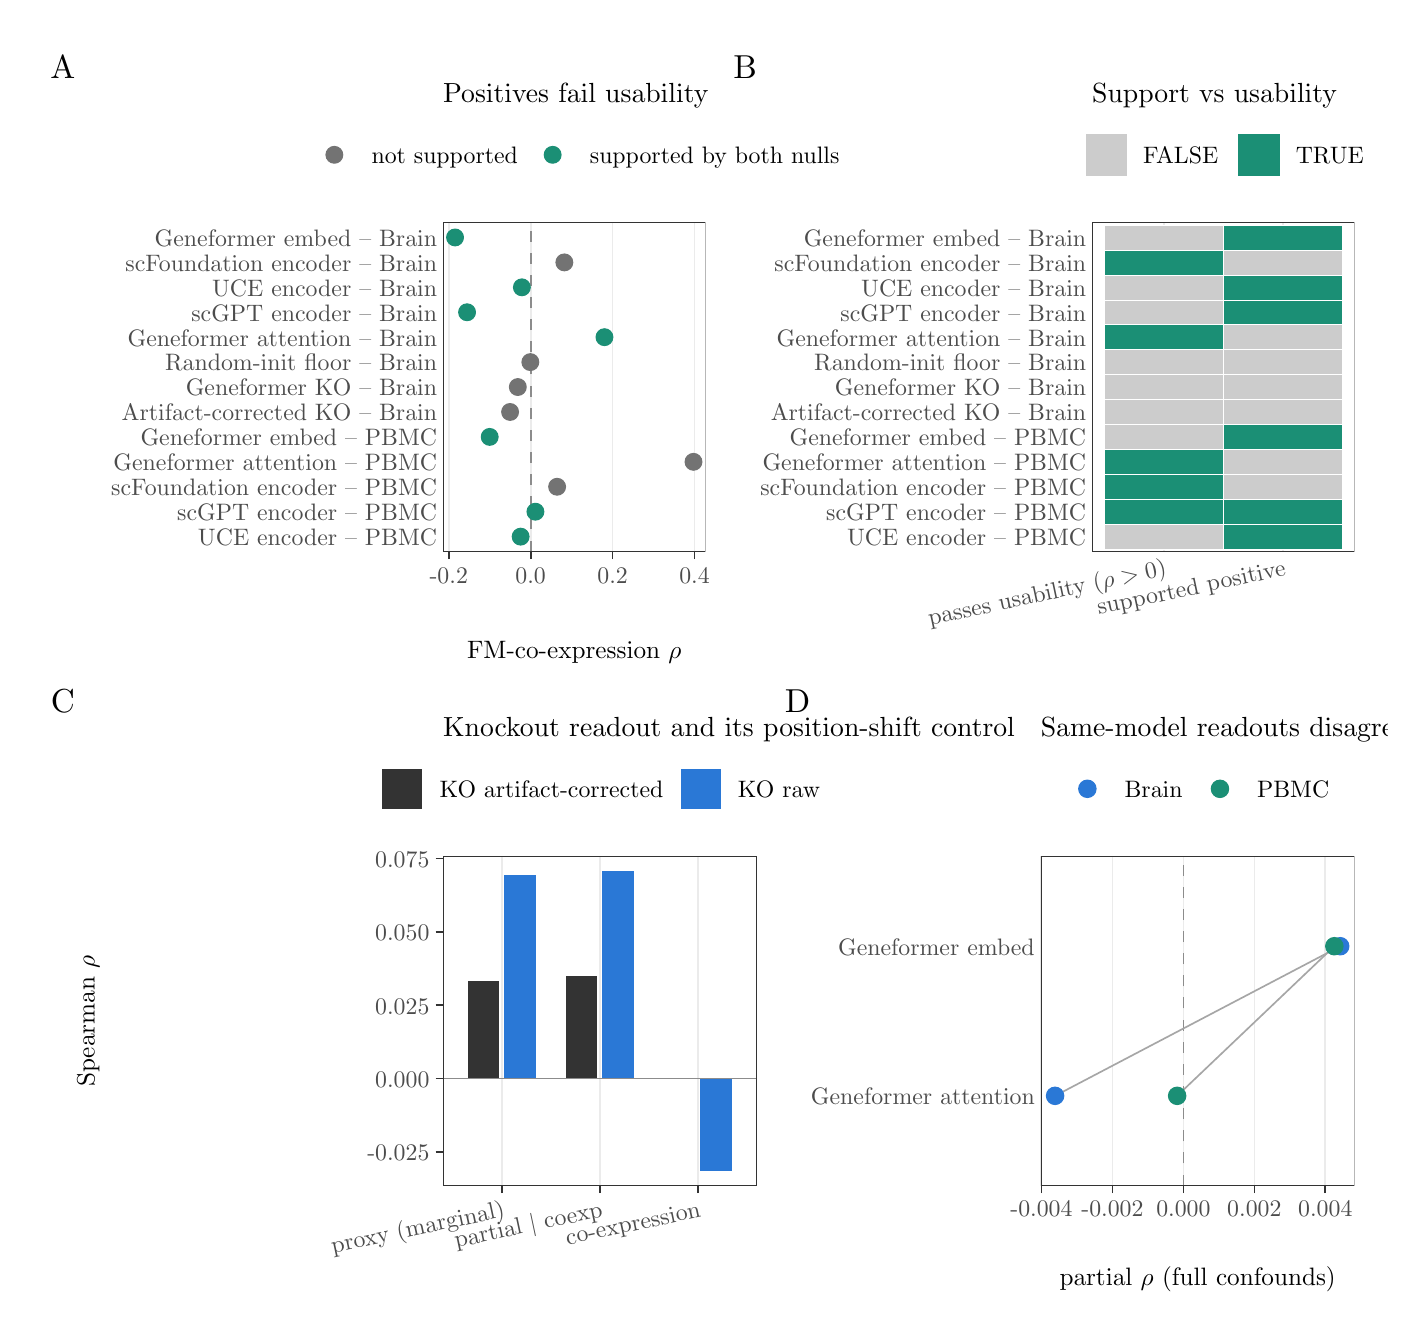
\begin{tikzpicture}[x=1pt,y=1pt]
\definecolor{fillColor}{RGB}{255,255,255}
\path[use as bounding box,fill=fillColor,fill opacity=0.00] (0,0) rectangle (491.44,462.53);
\begin{scope}
\path[clip] (  0.00,  0.00) rectangle (491.44,462.53);
\definecolor{drawColor}{RGB}{255,255,255}
\definecolor{fillColor}{RGB}{255,255,255}

\path[draw=drawColor,line width= 0.6pt,line join=round,line cap=round,fill=fillColor] ( -0.00,  0.00) rectangle (491.44,462.53);
\end{scope}
\begin{scope}
\path[clip] (  4.00,229.44) rectangle (250.90,458.53);
\definecolor{drawColor}{RGB}{255,255,255}
\definecolor{fillColor}{RGB}{255,255,255}

\path[draw=drawColor,line width= 0.6pt,line join=round,line cap=round,fill=fillColor] (  4.00,229.44) rectangle (250.90,458.53);
\end{scope}
\begin{scope}
\path[clip] (250.90,229.44) rectangle (485.44,458.53);
\definecolor{drawColor}{RGB}{255,255,255}
\definecolor{fillColor}{RGB}{255,255,255}

\path[draw=drawColor,line width= 0.6pt,line join=round,line cap=round,fill=fillColor] (250.90,229.44) rectangle (485.44,458.53);
\end{scope}
\begin{scope}
\path[clip] (150.12,273.20) rectangle (244.90,392.13);
\definecolor{fillColor}{RGB}{255,255,255}

\path[fill=fillColor] (150.12,273.20) rectangle (244.90,392.13);
\definecolor{drawColor}{gray}{0.92}

\path[draw=drawColor,line width= 0.6pt,line join=round] (152.15,273.20) --
	(152.15,392.13);

\path[draw=drawColor,line width= 0.6pt,line join=round] (181.76,273.20) --
	(181.76,392.13);

\path[draw=drawColor,line width= 0.6pt,line join=round] (211.37,273.20) --
	(211.37,392.13);

\path[draw=drawColor,line width= 0.6pt,line join=round] (240.97,273.20) --
	(240.97,392.13);
\definecolor{drawColor}{gray}{0.55}

\path[draw=drawColor,line width= 0.6pt,dash pattern=on 4pt off 4pt ,line join=round] (181.76,273.20) -- (181.76,392.13);
\definecolor{drawColor}{RGB}{27,143,117}
\definecolor{fillColor}{RGB}{27,143,117}

\path[draw=drawColor,line width= 0.4pt,line join=round,line cap=round,fill=fillColor] (154.43,386.72) circle (  3.03);
\definecolor{drawColor}{gray}{0.45}
\definecolor{fillColor}{gray}{0.45}

\path[draw=drawColor,line width= 0.4pt,line join=round,line cap=round,fill=fillColor] (193.93,377.71) circle (  3.03);
\definecolor{drawColor}{RGB}{27,143,117}
\definecolor{fillColor}{RGB}{27,143,117}

\path[draw=drawColor,line width= 0.4pt,line join=round,line cap=round,fill=fillColor] (178.58,368.70) circle (  3.03);

\path[draw=drawColor,line width= 0.4pt,line join=round,line cap=round,fill=fillColor] (158.77,359.69) circle (  3.03);

\path[draw=drawColor,line width= 0.4pt,line join=round,line cap=round,fill=fillColor] (208.42,350.69) circle (  3.03);
\definecolor{drawColor}{gray}{0.45}
\definecolor{fillColor}{gray}{0.45}

\path[draw=drawColor,line width= 0.4pt,line join=round,line cap=round,fill=fillColor] (181.64,341.68) circle (  3.03);

\path[draw=drawColor,line width= 0.4pt,line join=round,line cap=round,fill=fillColor] (177.11,332.67) circle (  3.03);

\path[draw=drawColor,line width= 0.4pt,line join=round,line cap=round,fill=fillColor] (174.32,323.66) circle (  3.03);
\definecolor{drawColor}{RGB}{27,143,117}
\definecolor{fillColor}{RGB}{27,143,117}

\path[draw=drawColor,line width= 0.4pt,line join=round,line cap=round,fill=fillColor] (166.95,314.65) circle (  3.03);
\definecolor{drawColor}{gray}{0.45}
\definecolor{fillColor}{gray}{0.45}

\path[draw=drawColor,line width= 0.4pt,line join=round,line cap=round,fill=fillColor] (240.59,305.64) circle (  3.03);

\path[draw=drawColor,line width= 0.4pt,line join=round,line cap=round,fill=fillColor] (191.31,296.63) circle (  3.03);
\definecolor{drawColor}{RGB}{27,143,117}
\definecolor{fillColor}{RGB}{27,143,117}

\path[draw=drawColor,line width= 0.4pt,line join=round,line cap=round,fill=fillColor] (183.47,287.62) circle (  3.03);

\path[draw=drawColor,line width= 0.4pt,line join=round,line cap=round,fill=fillColor] (178.13,278.61) circle (  3.03);
\definecolor{drawColor}{gray}{0.20}

\path[draw=drawColor,line width= 0.6pt,line join=round,line cap=round] (150.12,273.20) rectangle (244.90,392.13);
\end{scope}
\begin{scope}
\path[clip] (  0.00,  0.00) rectangle (491.44,462.53);
\definecolor{drawColor}{gray}{0.30}

\node[text=drawColor,anchor=base east,inner sep=0pt, outer sep=0pt, scale=  0.86] at (147.92,275.41) {UCE encoder -- PBMC};

\node[text=drawColor,anchor=base east,inner sep=0pt, outer sep=0pt, scale=  0.86] at (147.92,284.42) {scGPT encoder -- PBMC};

\node[text=drawColor,anchor=base east,inner sep=0pt, outer sep=0pt, scale=  0.86] at (147.92,293.43) {scFoundation encoder -- PBMC};

\node[text=drawColor,anchor=base east,inner sep=0pt, outer sep=0pt, scale=  0.86] at (147.92,302.44) {Geneformer attention -- PBMC};

\node[text=drawColor,anchor=base east,inner sep=0pt, outer sep=0pt, scale=  0.86] at (147.92,311.45) {Geneformer embed -- PBMC};

\node[text=drawColor,anchor=base east,inner sep=0pt, outer sep=0pt, scale=  0.86] at (147.92,320.46) {Artifact-corrected KO -- Brain};

\node[text=drawColor,anchor=base east,inner sep=0pt, outer sep=0pt, scale=  0.86] at (147.92,329.47) {Geneformer KO -- Brain};

\node[text=drawColor,anchor=base east,inner sep=0pt, outer sep=0pt, scale=  0.86] at (147.92,338.48) {Random-init floor -- Brain};

\node[text=drawColor,anchor=base east,inner sep=0pt, outer sep=0pt, scale=  0.86] at (147.92,347.49) {Geneformer attention -- Brain};

\node[text=drawColor,anchor=base east,inner sep=0pt, outer sep=0pt, scale=  0.86] at (147.92,356.50) {scGPT encoder -- Brain};

\node[text=drawColor,anchor=base east,inner sep=0pt, outer sep=0pt, scale=  0.86] at (147.92,365.51) {UCE encoder -- Brain};

\node[text=drawColor,anchor=base east,inner sep=0pt, outer sep=0pt, scale=  0.86] at (147.92,374.52) {scFoundation encoder -- Brain};

\node[text=drawColor,anchor=base east,inner sep=0pt, outer sep=0pt, scale=  0.86] at (147.92,383.53) {Geneformer embed -- Brain};
\end{scope}
\begin{scope}
\path[clip] (  0.00,  0.00) rectangle (491.44,462.53);
\definecolor{drawColor}{gray}{0.20}

\path[draw=drawColor,line width= 0.6pt,line join=round] (152.15,270.45) --
	(152.15,273.20);

\path[draw=drawColor,line width= 0.6pt,line join=round] (181.76,270.45) --
	(181.76,273.20);

\path[draw=drawColor,line width= 0.6pt,line join=round] (211.37,270.45) --
	(211.37,273.20);

\path[draw=drawColor,line width= 0.6pt,line join=round] (240.97,270.45) --
	(240.97,273.20);
\end{scope}
\begin{scope}
\path[clip] (  0.00,  0.00) rectangle (491.44,462.53);
\definecolor{drawColor}{gray}{0.30}

\node[text=drawColor,anchor=base,inner sep=0pt, outer sep=0pt, scale=  0.86] at (152.15,261.86) {-0.2};

\node[text=drawColor,anchor=base,inner sep=0pt, outer sep=0pt, scale=  0.86] at (181.76,261.86) {0.0};

\node[text=drawColor,anchor=base,inner sep=0pt, outer sep=0pt, scale=  0.86] at (211.37,261.86) {0.2};

\node[text=drawColor,anchor=base,inner sep=0pt, outer sep=0pt, scale=  0.86] at (240.97,261.86) {0.4};
\end{scope}
\begin{scope}
\path[clip] (  0.00,  0.00) rectangle (491.44,462.53);
\definecolor{drawColor}{RGB}{0,0,0}

\node[text=drawColor,anchor=base,inner sep=0pt, outer sep=0pt, scale=  0.91] at (197.51,234.60) {FM-co-expression $\rho$};
\end{scope}
\begin{scope}
\path[clip] (  0.00,  0.00) rectangle (491.44,462.53);
\definecolor{fillColor}{RGB}{255,255,255}

\path[fill=fillColor] ( 97.37,403.13) rectangle (297.65,430.03);
\end{scope}
\begin{scope}
\path[clip] (  0.00,  0.00) rectangle (491.44,462.53);
\definecolor{fillColor}{RGB}{255,255,255}

\path[fill=fillColor] (102.87,408.63) rectangle (118.77,424.53);
\definecolor{drawColor}{gray}{0.45}
\definecolor{fillColor}{gray}{0.45}

\path[draw=drawColor,line width= 0.4pt,line join=round,line cap=round,fill=fillColor] (110.82,416.58) circle (  3.03);
\end{scope}
\begin{scope}
\path[clip] (  0.00,  0.00) rectangle (491.44,462.53);
\definecolor{fillColor}{RGB}{255,255,255}

\path[fill=fillColor] (181.75,408.63) rectangle (197.65,424.53);
\definecolor{drawColor}{RGB}{27,143,117}
\definecolor{fillColor}{RGB}{27,143,117}

\path[draw=drawColor,line width= 0.4pt,line join=round,line cap=round,fill=fillColor] (189.70,416.58) circle (  3.03);
\end{scope}
\begin{scope}
\path[clip] (  0.00,  0.00) rectangle (491.44,462.53);
\definecolor{drawColor}{RGB}{0,0,0}

\node[text=drawColor,anchor=base west,inner sep=0pt, outer sep=0pt, scale=  0.86] at (124.27,413.38) {not supported};
\end{scope}
\begin{scope}
\path[clip] (  0.00,  0.00) rectangle (491.44,462.53);
\definecolor{drawColor}{RGB}{0,0,0}

\node[text=drawColor,anchor=base west,inner sep=0pt, outer sep=0pt, scale=  0.86] at (203.15,413.38) {supported by both nulls};
\end{scope}
\begin{scope}
\path[clip] (  0.00,  0.00) rectangle (491.44,462.53);
\definecolor{drawColor}{RGB}{0,0,0}

\node[text=drawColor,anchor=base west,inner sep=0pt, outer sep=0pt, scale=  1.00] at (150.12,435.40) {Positives fail usability};
\end{scope}
\begin{scope}
\path[clip] (  0.00,  0.00) rectangle (491.44,462.53);
\definecolor{drawColor}{RGB}{0,0,0}

\node[text=drawColor,anchor=base,inner sep=0pt, outer sep=0pt, scale=  1.20] at ( 12.74,444.22) {A};
\end{scope}
\begin{scope}
\path[clip] (384.66,273.20) rectangle (479.44,392.13);
\definecolor{fillColor}{RGB}{255,255,255}

\path[fill=fillColor] (384.66,273.20) rectangle (479.44,392.13);
\definecolor{drawColor}{gray}{0.92}

\path[draw=drawColor,line width= 0.6pt,line join=round] (410.51,273.20) --
	(410.51,392.13);

\path[draw=drawColor,line width= 0.6pt,line join=round] (453.59,273.20) --
	(453.59,392.13);
\definecolor{drawColor}{RGB}{255,255,255}
\definecolor{fillColor}{RGB}{27,143,117}

\path[draw=drawColor,line width= 0.2pt,fill=fillColor] (432.05,382.22) rectangle (475.13,391.23);
\definecolor{fillColor}{gray}{0.80}

\path[draw=drawColor,line width= 0.2pt,fill=fillColor] (432.05,373.21) rectangle (475.13,382.22);
\definecolor{fillColor}{RGB}{27,143,117}

\path[draw=drawColor,line width= 0.2pt,fill=fillColor] (432.05,364.20) rectangle (475.13,373.21);

\path[draw=drawColor,line width= 0.2pt,fill=fillColor] (432.05,355.19) rectangle (475.13,364.20);
\definecolor{fillColor}{gray}{0.80}

\path[draw=drawColor,line width= 0.2pt,fill=fillColor] (432.05,346.18) rectangle (475.13,355.19);

\path[draw=drawColor,line width= 0.2pt,fill=fillColor] (432.05,337.17) rectangle (475.13,346.18);

\path[draw=drawColor,line width= 0.2pt,fill=fillColor] (432.05,328.16) rectangle (475.13,337.17);

\path[draw=drawColor,line width= 0.2pt,fill=fillColor] (432.05,319.15) rectangle (475.13,328.16);
\definecolor{fillColor}{RGB}{27,143,117}

\path[draw=drawColor,line width= 0.2pt,fill=fillColor] (432.05,310.14) rectangle (475.13,319.15);
\definecolor{fillColor}{gray}{0.80}

\path[draw=drawColor,line width= 0.2pt,fill=fillColor] (432.05,301.13) rectangle (475.13,310.14);

\path[draw=drawColor,line width= 0.2pt,fill=fillColor] (432.05,292.12) rectangle (475.13,301.13);
\definecolor{fillColor}{RGB}{27,143,117}

\path[draw=drawColor,line width= 0.2pt,fill=fillColor] (432.05,283.11) rectangle (475.13,292.12);

\path[draw=drawColor,line width= 0.2pt,fill=fillColor] (432.05,274.10) rectangle (475.13,283.11);
\definecolor{fillColor}{gray}{0.80}

\path[draw=drawColor,line width= 0.2pt,fill=fillColor] (388.97,382.22) rectangle (432.05,391.23);
\definecolor{fillColor}{RGB}{27,143,117}

\path[draw=drawColor,line width= 0.2pt,fill=fillColor] (388.97,373.21) rectangle (432.05,382.22);
\definecolor{fillColor}{gray}{0.80}

\path[draw=drawColor,line width= 0.2pt,fill=fillColor] (388.97,364.20) rectangle (432.05,373.21);

\path[draw=drawColor,line width= 0.2pt,fill=fillColor] (388.97,355.19) rectangle (432.05,364.20);
\definecolor{fillColor}{RGB}{27,143,117}

\path[draw=drawColor,line width= 0.2pt,fill=fillColor] (388.97,346.18) rectangle (432.05,355.19);
\definecolor{fillColor}{gray}{0.80}

\path[draw=drawColor,line width= 0.2pt,fill=fillColor] (388.97,337.17) rectangle (432.05,346.18);

\path[draw=drawColor,line width= 0.2pt,fill=fillColor] (388.97,328.16) rectangle (432.05,337.17);

\path[draw=drawColor,line width= 0.2pt,fill=fillColor] (388.97,319.15) rectangle (432.05,328.16);

\path[draw=drawColor,line width= 0.2pt,fill=fillColor] (388.97,310.14) rectangle (432.05,319.15);
\definecolor{fillColor}{RGB}{27,143,117}

\path[draw=drawColor,line width= 0.2pt,fill=fillColor] (388.97,301.13) rectangle (432.05,310.14);

\path[draw=drawColor,line width= 0.2pt,fill=fillColor] (388.97,292.12) rectangle (432.05,301.13);

\path[draw=drawColor,line width= 0.2pt,fill=fillColor] (388.97,283.11) rectangle (432.05,292.12);
\definecolor{fillColor}{gray}{0.80}

\path[draw=drawColor,line width= 0.2pt,fill=fillColor] (388.97,274.10) rectangle (432.05,283.11);
\definecolor{drawColor}{gray}{0.20}

\path[draw=drawColor,line width= 0.6pt,line join=round,line cap=round] (384.66,273.20) rectangle (479.44,392.13);
\end{scope}
\begin{scope}
\path[clip] (  0.00,  0.00) rectangle (491.44,462.53);
\definecolor{drawColor}{gray}{0.30}

\node[text=drawColor,anchor=base east,inner sep=0pt, outer sep=0pt, scale=  0.86] at (382.46,275.41) {UCE encoder -- PBMC};

\node[text=drawColor,anchor=base east,inner sep=0pt, outer sep=0pt, scale=  0.86] at (382.46,284.42) {scGPT encoder -- PBMC};

\node[text=drawColor,anchor=base east,inner sep=0pt, outer sep=0pt, scale=  0.86] at (382.46,293.43) {scFoundation encoder -- PBMC};

\node[text=drawColor,anchor=base east,inner sep=0pt, outer sep=0pt, scale=  0.86] at (382.46,302.44) {Geneformer attention -- PBMC};

\node[text=drawColor,anchor=base east,inner sep=0pt, outer sep=0pt, scale=  0.86] at (382.46,311.45) {Geneformer embed -- PBMC};

\node[text=drawColor,anchor=base east,inner sep=0pt, outer sep=0pt, scale=  0.86] at (382.46,320.46) {Artifact-corrected KO -- Brain};

\node[text=drawColor,anchor=base east,inner sep=0pt, outer sep=0pt, scale=  0.86] at (382.46,329.47) {Geneformer KO -- Brain};

\node[text=drawColor,anchor=base east,inner sep=0pt, outer sep=0pt, scale=  0.86] at (382.46,338.48) {Random-init floor -- Brain};

\node[text=drawColor,anchor=base east,inner sep=0pt, outer sep=0pt, scale=  0.86] at (382.46,347.49) {Geneformer attention -- Brain};

\node[text=drawColor,anchor=base east,inner sep=0pt, outer sep=0pt, scale=  0.86] at (382.46,356.50) {scGPT encoder -- Brain};

\node[text=drawColor,anchor=base east,inner sep=0pt, outer sep=0pt, scale=  0.86] at (382.46,365.51) {UCE encoder -- Brain};

\node[text=drawColor,anchor=base east,inner sep=0pt, outer sep=0pt, scale=  0.86] at (382.46,374.52) {scFoundation encoder -- Brain};

\node[text=drawColor,anchor=base east,inner sep=0pt, outer sep=0pt, scale=  0.86] at (382.46,383.53) {Geneformer embed -- Brain};
\end{scope}
\begin{scope}
\path[clip] (  0.00,  0.00) rectangle (491.44,462.53);
\definecolor{drawColor}{gray}{0.30}

\node[text=drawColor,rotate= 12.00,anchor=base east,inner sep=0pt, outer sep=0pt, scale=  0.86] at (411.84,264.75) {passes usability ($\rho>0$)};

\node[text=drawColor,rotate= 12.00,anchor=base east,inner sep=0pt, outer sep=0pt, scale=  0.86] at (454.92,264.75) {supported positive};
\end{scope}
\begin{scope}
\path[clip] (  0.00,  0.00) rectangle (491.44,462.53);
\definecolor{fillColor}{RGB}{255,255,255}

\path[fill=fillColor] (376.20,403.13) rectangle (487.90,430.03);
\end{scope}
\begin{scope}
\path[clip] (  0.00,  0.00) rectangle (491.44,462.53);
\definecolor{fillColor}{RGB}{255,255,255}

\path[fill=fillColor] (381.70,408.63) rectangle (397.60,424.53);
\definecolor{drawColor}{RGB}{255,255,255}
\definecolor{fillColor}{gray}{0.80}

\path[draw=drawColor,line width= 0.2pt,fill=fillColor] (381.98,408.91) rectangle (397.31,424.24);
\end{scope}
\begin{scope}
\path[clip] (  0.00,  0.00) rectangle (491.44,462.53);
\definecolor{fillColor}{RGB}{255,255,255}

\path[fill=fillColor] (436.83,408.63) rectangle (452.73,424.53);
\definecolor{drawColor}{RGB}{255,255,255}
\definecolor{fillColor}{RGB}{27,143,117}

\path[draw=drawColor,line width= 0.2pt,fill=fillColor] (437.12,408.91) rectangle (452.45,424.24);
\end{scope}
\begin{scope}
\path[clip] (  0.00,  0.00) rectangle (491.44,462.53);
\definecolor{drawColor}{RGB}{0,0,0}

\node[text=drawColor,anchor=base west,inner sep=0pt, outer sep=0pt, scale=  0.86] at (403.10,413.38) {FALSE};
\end{scope}
\begin{scope}
\path[clip] (  0.00,  0.00) rectangle (491.44,462.53);
\definecolor{drawColor}{RGB}{0,0,0}

\node[text=drawColor,anchor=base west,inner sep=0pt, outer sep=0pt, scale=  0.86] at (458.23,413.38) {TRUE};
\end{scope}
\begin{scope}
\path[clip] (  0.00,  0.00) rectangle (491.44,462.53);
\definecolor{drawColor}{RGB}{0,0,0}

\node[text=drawColor,anchor=base west,inner sep=0pt, outer sep=0pt, scale=  1.00] at (384.66,435.40) {Support vs usability};
\end{scope}
\begin{scope}
\path[clip] (  0.00,  0.00) rectangle (491.44,462.53);
\definecolor{drawColor}{RGB}{0,0,0}

\node[text=drawColor,anchor=base,inner sep=0pt, outer sep=0pt, scale=  1.20] at (259.28,444.22) {B};
\end{scope}
\begin{scope}
\path[clip] (  4.00,  3.00) rectangle (269.46,229.44);
\definecolor{drawColor}{RGB}{255,255,255}
\definecolor{fillColor}{RGB}{255,255,255}

\path[draw=drawColor,line width= 0.6pt,line join=round,line cap=round,fill=fillColor] (  4.00,  3.00) rectangle (269.46,229.44);
\end{scope}
\begin{scope}
\path[clip] (269.46,  3.00) rectangle (485.44,229.44);
\definecolor{drawColor}{RGB}{255,255,255}
\definecolor{fillColor}{RGB}{255,255,255}

\path[draw=drawColor,line width= 0.6pt,line join=round,line cap=round,fill=fillColor] (269.46,  3.00) rectangle (485.44,229.44);
\end{scope}
\begin{scope}
\path[clip] (150.12, 44.12) rectangle (263.46,163.04);
\definecolor{fillColor}{RGB}{255,255,255}

\path[fill=fillColor] (150.12, 44.12) rectangle (263.46,163.04);
\definecolor{drawColor}{gray}{0.92}

\path[draw=drawColor,line width= 0.6pt,line join=round] (171.37, 44.12) --
	(171.37,163.04);

\path[draw=drawColor,line width= 0.6pt,line join=round] (206.79, 44.12) --
	(206.79,163.04);

\path[draw=drawColor,line width= 0.6pt,line join=round] (242.21, 44.12) --
	(242.21,163.04);
\definecolor{fillColor}{RGB}{42,120,214}

\path[fill=fillColor] (172.26, 82.81) rectangle (183.77,156.26);

\path[fill=fillColor] (207.68, 82.81) rectangle (219.19,157.64);

\path[fill=fillColor] (243.09, 49.52) rectangle (254.60, 82.81);
\definecolor{fillColor}{gray}{0.20}

\path[fill=fillColor] (158.98, 82.81) rectangle (170.49,117.89);

\path[fill=fillColor] (194.39, 82.81) rectangle (205.90,120.01);
\definecolor{drawColor}{gray}{0.55}

\path[draw=drawColor,line width= 0.6pt,line join=round] (150.12, 82.81) -- (263.46, 82.81);
\definecolor{drawColor}{gray}{0.20}

\path[draw=drawColor,line width= 0.6pt,line join=round,line cap=round] (150.12, 44.12) rectangle (263.46,163.04);
\end{scope}
\begin{scope}
\path[clip] (  0.00,  0.00) rectangle (491.44,462.53);
\definecolor{drawColor}{gray}{0.30}

\node[text=drawColor,anchor=base east,inner sep=0pt, outer sep=0pt, scale=  0.86] at (145.17, 53.11) {-0.025};

\node[text=drawColor,anchor=base east,inner sep=0pt, outer sep=0pt, scale=  0.86] at (145.17, 79.61) {0.000};

\node[text=drawColor,anchor=base east,inner sep=0pt, outer sep=0pt, scale=  0.86] at (145.17,106.11) {0.025};

\node[text=drawColor,anchor=base east,inner sep=0pt, outer sep=0pt, scale=  0.86] at (145.17,132.61) {0.050};

\node[text=drawColor,anchor=base east,inner sep=0pt, outer sep=0pt, scale=  0.86] at (145.17,159.11) {0.075};
\end{scope}
\begin{scope}
\path[clip] (  0.00,  0.00) rectangle (491.44,462.53);
\definecolor{drawColor}{gray}{0.20}

\path[draw=drawColor,line width= 0.6pt,line join=round] (147.37, 56.31) --
	(150.12, 56.31);

\path[draw=drawColor,line width= 0.6pt,line join=round] (147.37, 82.81) --
	(150.12, 82.81);

\path[draw=drawColor,line width= 0.6pt,line join=round] (147.37,109.30) --
	(150.12,109.30);

\path[draw=drawColor,line width= 0.6pt,line join=round] (147.37,135.80) --
	(150.12,135.80);

\path[draw=drawColor,line width= 0.6pt,line join=round] (147.37,162.30) --
	(150.12,162.30);
\end{scope}
\begin{scope}
\path[clip] (  0.00,  0.00) rectangle (491.44,462.53);
\definecolor{drawColor}{gray}{0.20}

\path[draw=drawColor,line width= 0.6pt,line join=round] (171.37, 41.37) --
	(171.37, 44.12);

\path[draw=drawColor,line width= 0.6pt,line join=round] (206.79, 41.37) --
	(206.79, 44.12);

\path[draw=drawColor,line width= 0.6pt,line join=round] (242.21, 41.37) --
	(242.21, 44.12);
\end{scope}
\begin{scope}
\path[clip] (  0.00,  0.00) rectangle (491.44,462.53);
\definecolor{drawColor}{gray}{0.30}

\node[text=drawColor,rotate= 12.00,anchor=base east,inner sep=0pt, outer sep=0pt, scale=  0.86] at (172.70, 32.92) {proxy (marginal)};

\node[text=drawColor,rotate= 12.00,anchor=base east,inner sep=0pt, outer sep=0pt, scale=  0.86] at (208.12, 32.92) {partial $|$ coexp};

\node[text=drawColor,rotate= 12.00,anchor=base east,inner sep=0pt, outer sep=0pt, scale=  0.86] at (243.54, 32.92) {co-expression};
\end{scope}
\begin{scope}
\path[clip] (  0.00,  0.00) rectangle (491.44,462.53);
\definecolor{drawColor}{RGB}{0,0,0}

\node[text=drawColor,rotate= 90.00,anchor=base,inner sep=0pt, outer sep=0pt, scale=  0.91] at ( 24.22,103.58) {Spearman $\rho$};
\end{scope}
\begin{scope}
\path[clip] (  0.00,  0.00) rectangle (491.44,462.53);
\definecolor{fillColor}{RGB}{255,255,255}

\path[fill=fillColor] (121.98,174.04) rectangle (291.60,200.94);
\end{scope}
\begin{scope}
\path[clip] (  0.00,  0.00) rectangle (491.44,462.53);
\definecolor{fillColor}{RGB}{255,255,255}

\path[fill=fillColor] (127.48,179.54) rectangle (143.38,195.44);
\definecolor{fillColor}{gray}{0.20}

\path[fill=fillColor] (128.19,180.25) rectangle (142.66,194.73);
\end{scope}
\begin{scope}
\path[clip] (  0.00,  0.00) rectangle (491.44,462.53);
\definecolor{fillColor}{RGB}{255,255,255}

\path[fill=fillColor] (235.27,179.54) rectangle (251.17,195.44);
\definecolor{fillColor}{RGB}{42,120,214}

\path[fill=fillColor] (235.98,180.25) rectangle (250.45,194.73);
\end{scope}
\begin{scope}
\path[clip] (  0.00,  0.00) rectangle (491.44,462.53);
\definecolor{drawColor}{RGB}{0,0,0}

\node[text=drawColor,anchor=base west,inner sep=0pt, outer sep=0pt, scale=  0.86] at (148.88,184.30) {KO artifact-corrected};
\end{scope}
\begin{scope}
\path[clip] (  0.00,  0.00) rectangle (491.44,462.53);
\definecolor{drawColor}{RGB}{0,0,0}

\node[text=drawColor,anchor=base west,inner sep=0pt, outer sep=0pt, scale=  0.86] at (256.67,184.30) {KO raw};
\end{scope}
\begin{scope}
\path[clip] (  0.00,  0.00) rectangle (491.44,462.53);
\definecolor{drawColor}{RGB}{0,0,0}

\node[text=drawColor,anchor=base west,inner sep=0pt, outer sep=0pt, scale=  1.00] at (150.12,206.31) {Knockout readout and its position-shift control};
\end{scope}
\begin{scope}
\path[clip] (  0.00,  0.00) rectangle (491.44,462.53);
\definecolor{drawColor}{RGB}{0,0,0}

\node[text=drawColor,anchor=base,inner sep=0pt, outer sep=0pt, scale=  1.20] at ( 12.74,215.14) {C};
\end{scope}
\begin{scope}
\path[clip] (366.10, 44.12) rectangle (479.44,163.04);
\definecolor{fillColor}{RGB}{255,255,255}

\path[fill=fillColor] (366.10, 44.12) rectangle (479.44,163.04);
\definecolor{drawColor}{gray}{0.92}

\path[draw=drawColor,line width= 0.6pt,line join=round] (366.33, 44.12) --
	(366.33,163.04);

\path[draw=drawColor,line width= 0.6pt,line join=round] (391.97, 44.12) --
	(391.97,163.04);

\path[draw=drawColor,line width= 0.6pt,line join=round] (417.61, 44.12) --
	(417.61,163.04);

\path[draw=drawColor,line width= 0.6pt,line join=round] (443.26, 44.12) --
	(443.26,163.04);

\path[draw=drawColor,line width= 0.6pt,line join=round] (468.90, 44.12) --
	(468.90,163.04);
\definecolor{drawColor}{gray}{0.55}

\path[draw=drawColor,line width= 0.6pt,dash pattern=on 4pt off 4pt ,line join=round] (417.61, 44.12) -- (417.61,163.04);
\definecolor{drawColor}{gray}{0.65}

\path[draw=drawColor,line width= 0.6pt,line join=round] (371.25, 76.55) --
	(474.28,130.61);

\path[draw=drawColor,line width= 0.6pt,line join=round] (415.36, 76.55) --
	(472.16,130.61);
\definecolor{drawColor}{RGB}{42,120,214}
\definecolor{fillColor}{RGB}{42,120,214}

\path[draw=drawColor,line width= 0.4pt,line join=round,line cap=round,fill=fillColor] (474.28,130.61) circle (  3.14);

\path[draw=drawColor,line width= 0.4pt,line join=round,line cap=round,fill=fillColor] (371.25, 76.55) circle (  3.14);
\definecolor{drawColor}{RGB}{27,143,117}
\definecolor{fillColor}{RGB}{27,143,117}

\path[draw=drawColor,line width= 0.4pt,line join=round,line cap=round,fill=fillColor] (472.16,130.61) circle (  3.14);

\path[draw=drawColor,line width= 0.4pt,line join=round,line cap=round,fill=fillColor] (415.36, 76.55) circle (  3.14);
\definecolor{drawColor}{gray}{0.20}

\path[draw=drawColor,line width= 0.6pt,line join=round,line cap=round] (366.10, 44.12) rectangle (479.44,163.04);
\end{scope}
\begin{scope}
\path[clip] (  0.00,  0.00) rectangle (491.44,462.53);
\definecolor{drawColor}{gray}{0.30}

\node[text=drawColor,anchor=base east,inner sep=0pt, outer sep=0pt, scale=  0.86] at (363.90, 73.36) {Geneformer attention};

\node[text=drawColor,anchor=base east,inner sep=0pt, outer sep=0pt, scale=  0.86] at (363.90,127.41) {Geneformer embed};
\end{scope}
\begin{scope}
\path[clip] (  0.00,  0.00) rectangle (491.44,462.53);
\definecolor{drawColor}{gray}{0.20}

\path[draw=drawColor,line width= 0.6pt,line join=round] (366.33, 41.37) --
	(366.33, 44.12);

\path[draw=drawColor,line width= 0.6pt,line join=round] (391.97, 41.37) --
	(391.97, 44.12);

\path[draw=drawColor,line width= 0.6pt,line join=round] (417.61, 41.37) --
	(417.61, 44.12);

\path[draw=drawColor,line width= 0.6pt,line join=round] (443.26, 41.37) --
	(443.26, 44.12);

\path[draw=drawColor,line width= 0.6pt,line join=round] (468.90, 41.37) --
	(468.90, 44.12);
\end{scope}
\begin{scope}
\path[clip] (  0.00,  0.00) rectangle (491.44,462.53);
\definecolor{drawColor}{gray}{0.30}

\node[text=drawColor,anchor=base,inner sep=0pt, outer sep=0pt, scale=  0.86] at (366.33, 32.78) {-0.004};

\node[text=drawColor,anchor=base,inner sep=0pt, outer sep=0pt, scale=  0.86] at (391.97, 32.78) {-0.002};

\node[text=drawColor,anchor=base,inner sep=0pt, outer sep=0pt, scale=  0.86] at (417.61, 32.78) {0.000};

\node[text=drawColor,anchor=base,inner sep=0pt, outer sep=0pt, scale=  0.86] at (443.26, 32.78) {0.002};

\node[text=drawColor,anchor=base,inner sep=0pt, outer sep=0pt, scale=  0.86] at (468.90, 32.78) {0.004};
\end{scope}
\begin{scope}
\path[clip] (  0.00,  0.00) rectangle (491.44,462.53);
\definecolor{drawColor}{RGB}{0,0,0}

\node[text=drawColor,anchor=base,inner sep=0pt, outer sep=0pt, scale=  0.91] at (422.77,  8.16) {partial $\rho$ (full confounds)};
\end{scope}
\begin{scope}
\path[clip] (  0.00,  0.00) rectangle (491.44,462.53);
\definecolor{fillColor}{RGB}{255,255,255}

\path[fill=fillColor] (369.47,174.04) rectangle (476.06,200.94);
\end{scope}
\begin{scope}
\path[clip] (  0.00,  0.00) rectangle (491.44,462.53);
\definecolor{fillColor}{RGB}{255,255,255}

\path[fill=fillColor] (374.97,179.54) rectangle (390.87,195.44);
\definecolor{drawColor}{RGB}{42,120,214}
\definecolor{fillColor}{RGB}{42,120,214}

\path[draw=drawColor,line width= 0.4pt,line join=round,line cap=round,fill=fillColor] (382.92,187.49) circle (  3.14);
\end{scope}
\begin{scope}
\path[clip] (  0.00,  0.00) rectangle (491.44,462.53);
\definecolor{fillColor}{RGB}{255,255,255}

\path[fill=fillColor] (422.88,179.54) rectangle (438.78,195.44);
\definecolor{drawColor}{RGB}{27,143,117}
\definecolor{fillColor}{RGB}{27,143,117}

\path[draw=drawColor,line width= 0.4pt,line join=round,line cap=round,fill=fillColor] (430.83,187.49) circle (  3.14);
\end{scope}
\begin{scope}
\path[clip] (  0.00,  0.00) rectangle (491.44,462.53);
\definecolor{drawColor}{RGB}{0,0,0}

\node[text=drawColor,anchor=base west,inner sep=0pt, outer sep=0pt, scale=  0.86] at (396.37,184.30) {Brain};
\end{scope}
\begin{scope}
\path[clip] (  0.00,  0.00) rectangle (491.44,462.53);
\definecolor{drawColor}{RGB}{0,0,0}

\node[text=drawColor,anchor=base west,inner sep=0pt, outer sep=0pt, scale=  0.86] at (444.28,184.30) {PBMC};
\end{scope}
\begin{scope}
\path[clip] (  0.00,  0.00) rectangle (491.44,462.53);
\definecolor{drawColor}{RGB}{0,0,0}

\node[text=drawColor,anchor=base west,inner sep=0pt, outer sep=0pt, scale=  1.00] at (366.10,206.31) {Same-model readouts disagree};
\end{scope}
\begin{scope}
\path[clip] (  0.00,  0.00) rectangle (491.44,462.53);
\definecolor{drawColor}{RGB}{0,0,0}

\node[text=drawColor,anchor=base,inner sep=0pt, outer sep=0pt, scale=  1.20] at (278.20,215.14) {D};
\end{scope}
\end{tikzpicture}
